\documentclass{bmcart}

%%%%%%%%%%%%%%%%%%%%%%%%%%%%%%%%%%%%%%%%%%%%%%
%%                                          %%
%% CARGA DE PAQUETES DE LATEX               %%
%%                                          %%
%%%%%%%%%%%%%%%%%%%%%%%%%%%%%%%%%%%%%%%%%%%%%%

%%% Load packages
\usepackage{amsthm,amsmath}
\usepackage{graphicx}
%\RequirePackage[numbers]{natbib}
%\RequirePackage{hyperref}
\usepackage[utf8]{inputenc} %unicode support
%\usepackage[applemac]{inputenc} %applemac support if unicode package fails
%\usepackage[latin1]{inputenc} %UNIX support if unicode package fails


%%%%%%%%%%%%%%%%%%%%%%%%%%%%%%%%%%%%%%%%%%%%%%
%%                                          %%
%% COMIENZO DEL DOCUMENTO                   %%
%%                                          %%
%%%%%%%%%%%%%%%%%%%%%%%%%%%%%%%%%%%%%%%%%%%%%%

\begin{document}

	\begin{frontmatter}
	
		\begin{fmbox}
			\dochead{Research}
			
			%%%%%%%%%%%%%%%%%%%%%%%%%%%%%%%%%%%%%%%%%%%%%%
			%% INTRODUCIR TITULO PROYECTO               %%
			%%%%%%%%%%%%%%%%%%%%%%%%%%%%%%%%%%%%%%%%%%%%%%
			
			\title{A sample article title}
			
			%%%%%%%%%%%%%%%%%%%%%%%%%%%%%%%%%%%%%%%%%%%%%%
			%% AUTORES. METER UNA ENTRADA AUTHOR        %%
			%% POR PERSONA                              %%
			%%%%%%%%%%%%%%%%%%%%%%%%%%%%%%%%%%%%%%%%%%%%%%
			
			\author[
			  addressref={aff1},                   % ESTA LINEA SE COPIA IGUAL PARA CADA AUTOR
			  email={meixin3@uma.es}   % VUESTRO CORREO ACTIVO
			]{\inits{E.M.A.F}\fnm{Eva M.} \snm{Ayala Fernández}} % inits: INICIALES DE AUTOR, fnm: NOMBRE DE AUTOR, snm: APELLIDOS DE AUTOR
			\author[
			  addressref={aff1},
			  email={raulcastrov@uma.es}
			]{\inits{R.A.C.V.}\fnm{Raúl A.} \snm{Castro Valderas}}
				\author[
			addressref={aff1},
			email={mariajose.hidalgo@uma.es}
			]{\inits{M.J.H.R.}\fnm{María J.} \snm{Hidalgo Rodríguez}}
				\author[
			addressref={aff1},
			email={francisco.rodriguezcordoba@uma.es}
			]{\inits{F.J.R.L.}\fnm{Francisco J.} \snm{Rodríguez-cordoba Lucena}}
				\author[
			addressref={aff1},
			corref={aff1},                       % ESTA LINEA SOLO DEBE TENERLA EL COORDINADOR DEL GRUPO
			email={mariavida262001@uma.es}
			]{\inits{M.V.}\fnm{María} \snm{Vida Montañez}}
			
			%%%%%%%%%%%%%%%%%%%%%%%%%%%%%%%%%%%%%%%%%%%%%%
			%% AFILIACION. NO TOCAR                     %%
			%%%%%%%%%%%%%%%%%%%%%%%%%%%%%%%%%%%%%%%%%%%%%%
			
			\address[id=aff1]{%                           % unique id
			  \orgdiv{ETSI Informática},             % department, if any
			  \orgname{Universidad de Málaga},          % university, etc
			  \city{Málaga},                              % city
			  \cny{España}                                    % country
			}
		
		\end{fmbox}% comment this for two column layout
		
		\begin{abstractbox}
		
			\begin{abstract} % abstract
			
			%%%%%%%%%%%%%%%%%%%%%%%%%%%%%%%%%%%%%%%%%%%%%%%
			%% RESUMEN BREVE DE NO MAS DE 100 PALABRAS   %%
			%%%%%%%%%%%%%%%%%%%%%%%%%%%%%%%%%%%%%%%%%%%%%%%	
			
			\end{abstract}
			
			%%%%%%%%%%%%%%%%%%%%%%%%%%%%%%%%%%%%%%%%%%%%%%
			%% PALABRAS CLAVE DEL PROYECTO              %%
			%%%%%%%%%%%%%%%%%%%%%%%%%%%%%%%%%%%%%%%%%%%%%%
			
			\begin{keyword}
			\kwd{sample}
			\kwd{article}
			\kwd{author}
			\end{keyword}
		
		
		\end{abstractbox}
	
	\end{frontmatter}
	
	
	

	
	%%%%%%%%%%%%%%%%%%%%%%%%%%%%%%%%%
	%% COMIENZO DEL DOCUMENTO REAL %%
	%%%%%%%%%%%%%%%%%%%%%%%%%%%%%%%%%
	
	\section{Introducción}
Un papiloma es un tumor epitelial benigno que crece de manera exofítica \cite{Kozomara2007}, es decir, proyectándose hacia afuera en forma de proyecciones y de manera no agresiva ni propagándose por todo el cuerpo. En este contexto, "papila" se refiere a la proyección creada por el tumor, no a un tumor en una papila ya existente.
Cuando se utiliza sin contexto específico, con frecuencia se refiere a infecciones causadas por el virus del papiloma humano (VPH). Existen casi 200 tipos distintos de VPH \cite{Ljubojevic2014}, y muchos de ellos son carcinogénicos. Sin embargo, también existen otras condiciones que pueden causar papilomas, así como muchos casos en los que la causa no se conoce.
Las infecciones por el VPH de riesgo alto en ocasiones causan cáncer en las partes del cuerpo en las que el VPH infecta a las células. Por ejemplo, cáncer de cuello uterino, cáncer vulvar, cáncer vaginal, cáncer de pene, cáncer anal y cánceres orofaríngeos positivos para el VPH. La carga de los cánceres relacionados con el virus del papiloma humano causa cerca del 5\% \cite{papiloma} de todos los cánceres en el mundo, se calcula que 570.000 mujeres y 60.000 hombres tienen un cáncer relacionado con el VPH cada año \cite{papiloma} . El cáncer de cuello uterino es el más frecuente de todos los causados por el VPH, debido a que este es la causa de casi todos los cánceres de cuello uterino del mundo \cite{papiloma}.

\vspace{5pt}

\subsection{Información sobre los genes a estudiar} 
A continuación, veremos una breve información de los genes con mayor grado de interconexión que hemos encontrado al realizar un análisis fenotípico (HPO).

\vspace{3pt}

\textbf{AKT1}: La proteína kinasa B (AkT1) tiene un papel fundamental en el crecimiento y la supervivencia celular al transducir señales en la cascada de señalización celular (PI3K)/AKT, la cual genera mensajeros que participan en la regulación de la progresión del ciclo celular, adhesión y migración. La vía  PI3K/AKT es una de las que suelen estar afectadas en distintos tipos de cáncer en humanos, como el cáncer de ovario, de mama, y de cowden. Además, se asocia los niveles altos de fosforilación de la proteína con los peores pronósticos de cáncer \cite{Siegel2012}.

\textbf{TP53}: TP53 (tumor protein p53) es un gen supresor de tumores involucrado en procesos biológicos fundamentales para la estabilidad genética. Las mutaciones en este gen han sido asociadas con un peor pronóstico para pacientes con carcinoma oral de células escamosas, dando lugar a un cáncer más agresivo al combinarse con el VPH \cite{McKenna2021}.

\textbf{HRAS}: Este gen participa en la regulación de la vía de la proteína quinasa activada por mitógenos (MAPK) y mediada por la proteína quinasa Raf. En los últimos años se han definido una serie de síndromes con mutaciones en genes implicados en esta vía Ras/PAPK, entre ellos el síndrome de Costellos. Este síndrome refleja características cutáneas distintivas, como papillomas \cite{Siegel2012}.

\textbf{SDHD}: Las mutaciones en este gen están asociadas con la formación de tumores, incluyendo el paraganglioma hereditario. La transmisión de la enfermedad ocurre casi exclusivamente a través del alelo paterno, lo que sugiere que este locus puede estar impreso maternalmente. Hay pseudogenes para este gen en los cromosomas 1, 2, 3, 7 y 18. Resultados de empalme alternativos en múltiples variantes de transcripción \cite{Hensen2004}.

\textbf{SDHB}: Las mutaciones en este gen dan como resultado feocromocitoma y paraganglioma. Las alteraciones germinales y variaciones en este gen causan el síndrome de Cowden. Recientemente se ha reconocido el cáncer de endometrio como un componente importante de este síndrome \cite{Mahdi2015}.

\vspace{5pt}

\subsection{Hipótesis del trabajo}
Al mapear los genes asociados con el papiloma en una red de interacción proteína-proteína, podemos modelar este fenotipo y buscar grupos de genes que formen conglomerados dentro de la red. Al hacerlo, planteamos la hipótesis de que encontraremos grupos de genes involucrados en procesos subyacentes importantes relacionados con el crecimiento tumoral, y diversos cánceres como el de cuello uterino.


	\section{Materiales y métodos}

\subsection{Materiales}
A continuación, explicaremos los recursos y herramientas utilizados para los experimentos:

\vspace{3pt}

\textbf{Human Phenotype Ontology}\\ HPO es un vocabulario estandarizado de anomalías fenotípicas en enfermedades humanas que utiliza un fenotipado detallado para poder ser usado a nivel computacional \cite{HPO}.

\vspace{3pt}

\textbf{R}\\ R, en su esencia, es un lenguaje destinado a la exploración estadística y la creación de representaciones gráficas. Se configura como un entorno de programación compuesto por un conjunto de herramientas altamente adaptables, cuya funcionalidad puede ser expandida con facilidad a través de la integración de paquetes, bibliotecas o mediante la creación de funciones personalizadas. Además, se destaca por ser una plataforma de código abierto y gratuita, enmarcada en el proyecto GNU, compartiendo este enfoque con sistemas como Linux o aplicaciones como Mozilla Firefox. En nuestro caso hemos trabajado con la versión 4.3.1 de R \cite{Giorgi2022}.

\vspace{3pt}

\textbf{Python}\\
Python es un lenguaje de programación versátil de alto nivel ampliamente empleado en el desarrollo de diversas aplicaciones. A diferencia de lenguajes como Java o .NET, Python es interpretado, lo que significa que no requiere un proceso de compilación antes de ejecutar las aplicaciones. En lugar de eso, las aplicaciones escritas en Python se ejecutan directamente en la computadora utilizando un intérprete, eliminando la necesidad de traducción a lenguaje de máquina previamente. Este enfoque agiliza el desarrollo y ejecución de programas en Python. La versión utilizada de Python fue la 3.12.0 \cite{Mehare2023}.

\vspace{3pt}

\textbf{String}\\
String es una base de datos que alberga información sobre interacciones entre proteínas, tanto aquellas conocidas como las predichas. Estas interacciones abarcan desde asociaciones directas (físicas) hasta indirectas (funcionales). La base de datos recopila datos de diversas fuentes, que incluyen repositorios experimentales, métodos de predicción computacional y colecciones de textos públicos. Cada interacción está evaluada con una puntuación de condensación combinada que sintetiza las diversas evidencias disponibles\cite{Szklarczyk2021}.

\vspace{3pt}

\textbf{iGraph}\\
iGraph es una biblioteca rápida y de código abierto para el análisis de grafos o redes. El núcleo de esta librería está implementado en C y dispone de enlaces para su uso con lenguajes de alto nivel como R, Python y Mathematica \cite{Csardi2006}.

\vspace{3pt}

\textbf{Pandas}\\
Pandas es una biblioteca de programación en Python diseñada para facilitar el análisis y la manipulación de datos. Se centra en estructuras de datos como el "DataFrame", una tabla bidimensional, y ofrece funciones para cargar, limpiar y transformar datos de manera eficiente. Es ampliamente utilizado en ciencia de datos y análisis estadístico \cite{Snehkunj2022}.

\vspace{3pt}

\textbf{Algoritmos de clusterización}\\
Los algoritmos de clusterización son técnicas utilizadas en análisis de datos para dividir un conjunto de datos en grupos o "clústeres" basándose en similitudes entre los elementos. El objetivo es agrupar datos que sean más similares entre sí y más diferentes de otros grupos. Estos algoritmos ayudan a descubrir patrones y estructuras intrínsecas en los datos sin necesidad de etiquetas preexistentes. Los que se utilizaron para el trabajo fueron los siguientes:

•\textbf{Algoritmo de Givan-Newman}: es un método utilizado para detectar comunidades en redes complejas. Este algoritmo se basa en la idea de eliminar gradualmente los enlaces más importantes de una red para revelar su estructura de comunidad.

•\textbf{Algoritmo de optimización voraz}: también conocido como algoritmo ávido o greedy, es un enfoque de resolución de problemas que toma decisiones locales en cada etapa con la esperanza de encontrar una solución óptima global. En cada paso, el algoritmo selecciona la mejor opción disponible en ese momento, sin considerar las posibles consecuencias a largo plazo.

•\textbf{Algoritmo de propagación de etiquetas}: también conocido como "propagación de la afinidad," es un método de agrupamiento basado en la similitud entre los datos. A diferencia de otros algoritmos de agrupamiento que requieren la especificación del número de clústeres, la propagación de etiquetas es un algoritmo de agrupamiento sin la necesidad de definir previamente el número de clústeres.

•\textbf{Algoritmo de Louvain}: es un algoritmo de optimización utilizado para la detección de comunidades en redes o grafos. Su objetivo es encontrar una partición modular del grafo que maximice la modularidad. La modularidad es una medida que cuantifica la calidad de la partición de un grafo en comunidades, considerando la densidad de conexiones dentro de las comunidades y la rareza de conexiones entre ellas.

\vspace{3pt}

\textbf{Linkcomm}\\
Las comunidades de enlaces revelan la estructura anidada y superpuesta en las redes y descubren los nodos clave que forman conexiones con varias comunidades. Linkcomm proporciona un conjunto de herramientas para generar, visualizar y analizar comunidades de enlaces en redes de tamaño y tipo arbitrarios. El paquete linkcomm también incluye herramientas para generar, visualizar y analizar comunidades de Generadores de Clúster Superpuestos (OCG) \cite{Kalinka2011}.


\subsection{Métodos}
En primer lugar creamos una función que busca genes asociados a un fenotipo específico utilizando la API de \textbf{HPO}.
La función recibe el parámetro fenotipo, que es el código HPO para el fenotipo de interés.
Realizamos una solicitud GET a la API de HPO para obtener información sobre genes asociados al fenotipo.
Si la solicitud es exitosa (código de estado 200), extraemos y devolvemos los genes asociados al fenotipo. Si no, imprimimos un mensaje de error y devolvemos una lista vacía.


Utilizamos la función $buscar\_genes\_por\_fenotipo$ para obtener los genes asociados al fenotipo "Papilloma" (código HPO: HP:0012740).
Si encontramos genes asociados, imprimimos los nombres de los genes. Si no encontramos genes asociados, mostramos un mensaje indicando que no se encontraron genes.

Tras esto construimos una URL con los símbolos de los genes obtenidos anteriormente para realizar una solicitud a la API de StringDB, que proporciona información sobre interacciones de proteínas.
Realizamos una solicitud GET a la API de StringDB para obtener una red de interacciones de proteínas.
Guardamos la respuesta como una imagen llamada 'img.png'.

Imprimimos y filtramos los resultados del análisis de enriquecimiento por categorías ('Process' y 'KEGG').
Realizamos búsquedas específicas en los resultados de enfermedades y genes utilizando palabras clave y patrones de genes relevantes, respectivamente.
Guardamos los resultados de las búsquedas en archivos CSV .

Realizamos una solicitud GET a la API de StringDB para descargar la red de interacciones en formato TSV.
Si la descarga es exitosa, guardamos el archivo con el nombre proporcionado por la respuesta o como $'red_descargada.tsv'$ si no se obtiene un nombre de archivo.
Si hay un error en la descarga, imprimimos un mensaje de error.

Cargamos el archivo TSV descargado.
Seleccionamos columnas específicas ($'preferredName_A'$ y $'preferredName_B'$) y eliminamos duplicados.
Guardamos estas columnas en un nuevo archivo de texto llamado $'genes_igraph.txt'$.

\subsection{Propiedades de la red}

Nosotros usamos la biblioteca de \textbf{igraph} disponible en el lenguaje de programación de R para realizar el análisis y la visualización de la red. En primer lugar, importamos la librería y leímos el fichero que obtuvimos al generar la red con la API de STRINGDB y la guardamos en un grafo. A partir de este, estudiamos las \textbf{propiedades del grafo}, si todos los nodos estaban conectados con la función isconnected(), si era o no dirigido con la función is.directed(), el grado de centralidad que nos informaba del número de conexiones de cada gen con la función degree(), la centralidad de cercanía con la que obtuvimos la distancia promedio entre un nodo y todos los demás nodos mediante la aplicación de closeness(), y la conectividad que nos indicaba la fortaleza de la conexión del nodo aplicando $edge\_density()$. 

\vspace{3pt}
\subsection{Detección de comunidades}

En segundo lugar, llevamos a cabo la \textbf{identificación de comunidades} mediante distintos \textbf{algoritmos de clusterización}: método de Girvan-Newman, algoritmo de optimización voraz, propagación de etiquetas y el algoritmo de Louvain. 

\vspace{3pt}
\begin{enumerate}
\item El método de \textbf{Girvan Newman} (función $cluster_edge_betweenness()$, en el fichero $biologiasistemas_igraph.R$ en el repositorio GitHub del proyecto)detecta comunidades basándose en la centralidad de intermediación de los nodos, en otras palabras, va eliminando gradualmente las aristas más importantes para identificar las comunidades de la red \cite{Zahiri2023}.


\item El \textbf{algoritmo voraz} (función $cluster_fast_greedy()$, en el fichero $biologiasistemas_igraph.R$ en el repositorio GitHub del proyecto), busca formar grupos de datos de manera iterativa tomando en cada paso la elección más beneficiosa para fusionar o dividir clusters con el objetivo de maximizar un criterio local \cite{Curtis2003}.  


\item La \textbf{propagación de etiquetas} (función $cluster_label_prop()$, en el fichero $biologiasistemas_igraph.R$ en el repositorio GitHub del proyecto) es un enfoque basado en la difusión de información a través de la red que agrupa los nodos que están fuertemente conectados \cite{Garza2019}.

\item Por último el \textbf{algoritmo de Louvain} (función $cluster_louvain()$, en el fichero $biologiasistemas_igraph.R$ en el repositorio GitHub del proyecto)  busca organizar los nodos de una red en comunidades de manera que la modularidad global de la red sea máxima, o en otras palabras, cómo de bien se dividen los nodos de una red en grupos o comunidades distintas \cite{Zhang2021}.

\end{enumerate}

\vspace{3pt}

Para estudiar mejor a qué comunidad pertenece cada nodo, visualizamos el resultado de la aplicación del algoritmo de Louvain mediante la aplicación de \textbf{link communities} (función getLinkCommunities(), en el fichero $biologiasistemas_igraph.R$ en el repositorio GitHub del proyecto) que nos permitía identificar si alguno de los nodos se incluían en varias comunidades. 

\vspace{3pt}
\subsection{Interacción de genes de interés}

En tercer lugar, estudiamos la interacción de nuestros \textbf{genes de interés} especificados anteriormente: \textit{TP53}, \textit{HRAS}, \textit{AKT1}, \textit{SDHB}, \textit{SDHD}. Para ellos creamos una función (función $encontrar\_vecinos\_interesantes()$, en el fichero $biologiasistemas\_igraph.R$ en el repositorio GitHub del proyecto) que nos devolvía una tabla con los vecinos de cada uno de estos genes para saber si entre ellos estaban relacionados.

\vspace{3pt}

\subsection{Enriquecimiento funcional de la comunidad de interés.}

Tras estudiar la detección de comunidades optamos por realizar un enriquecimiento funcional de la comunidad en la que se encuentran nuestros genes de interés. Para ello, se busca la comunidad en la que se encuentran estos genes, se identifica esta y se guardan los genes que la conforman en el entorno de R. Esto lo hemos hecho con el comando \textit{ nodos\_genes\_interes \textless\ - V(net) \$name \%in\% genes\_interes} donde \textit{net} es nuestro grafo principal y $genes\_interes$ es un vector donde se encuentran definidos los genes de interés del estudio. Este comando encuentra los índices de los nodos que representan los genes de interés nuestro de nuestro grafo. Seguimos, obteniendo el índice de la comunidad que contiene estos genes de interés con el comando \textit{ cluster\_containing\_genes \textless\ - mermbership(cfg)[nodos\_genes\_interes]} donde $cfg$ es la variable donde se encuentran las diferentes comunidades que hemos identificado en nuestro grafo principal. Tras esto, con el comando \textit{genes\_cluster \textless\ - V(net)\$name[membership(cfg)==cluster\_containing\_genes]} guardamos todos los genes que conforman esta comunidad en una variable. Esta variable la guardamos en un fichero de texto con la función $write.table()$.

\vspace{3pt}

Una vez que tenemos el fichero de texto con los genes que conforman la comunidad de interés procedemos a realizar un enriquecimiento funcional. Para ello, en un nuevo script de Python que hemos llamado \textit{enriquecimiento\_cluster.py}. Comenzamos importando las librería necesarias y construyendo la URL para realizar una solicitud a la API de STRINGDB. Definimos la categoría funcional de interés, en nuestro caso HPO (para relacionar los genes con fenotipos patológicos), definimos la especie de nuestros genes, en este caso 9606 (referente a Homo Sapiens) y el archivo de genes donde se enucnetran nuestra comunidad de interés. Seguidamente recogemos los parámetros para el análisis funcional ya definidos en una solicitud a la API de StringDB. Creamos un dataframe con las columnas $Term, Preferred Name, Category, Description$ que muestran el término HPO, el nombre de los genes, la categoría funcional (en este caso, HPO) y una descripción del fenotipo patológico asociado.
Este dataset se guarda en un archivo csv con la función \textit{.to\_csv()}.

\vspace{3pt}

\subsection{Consulta de la relación entre genes asociados y fenotipos patológicos.}

Por último, hemos consultado manualmente el archivo csv creado con el dataframe anteriormente descrito y hemos identificado relaciones de genes asociados con fenotipos patológicos (estas consultas han sido filtradas por palabras clave como son: papiloma, genitales, renal, carcinoma, ovario y derivados, útero y derivados).



	
\section{Resultados}

\subsection{Red de interacción entre genes}

Se identificaron un total de 51 genes asociados al fenotipo \textbf{Papilloma} y obtuvimos una representación visual de la red de interacción entre los genes.
\begin{figure}
	\centering
	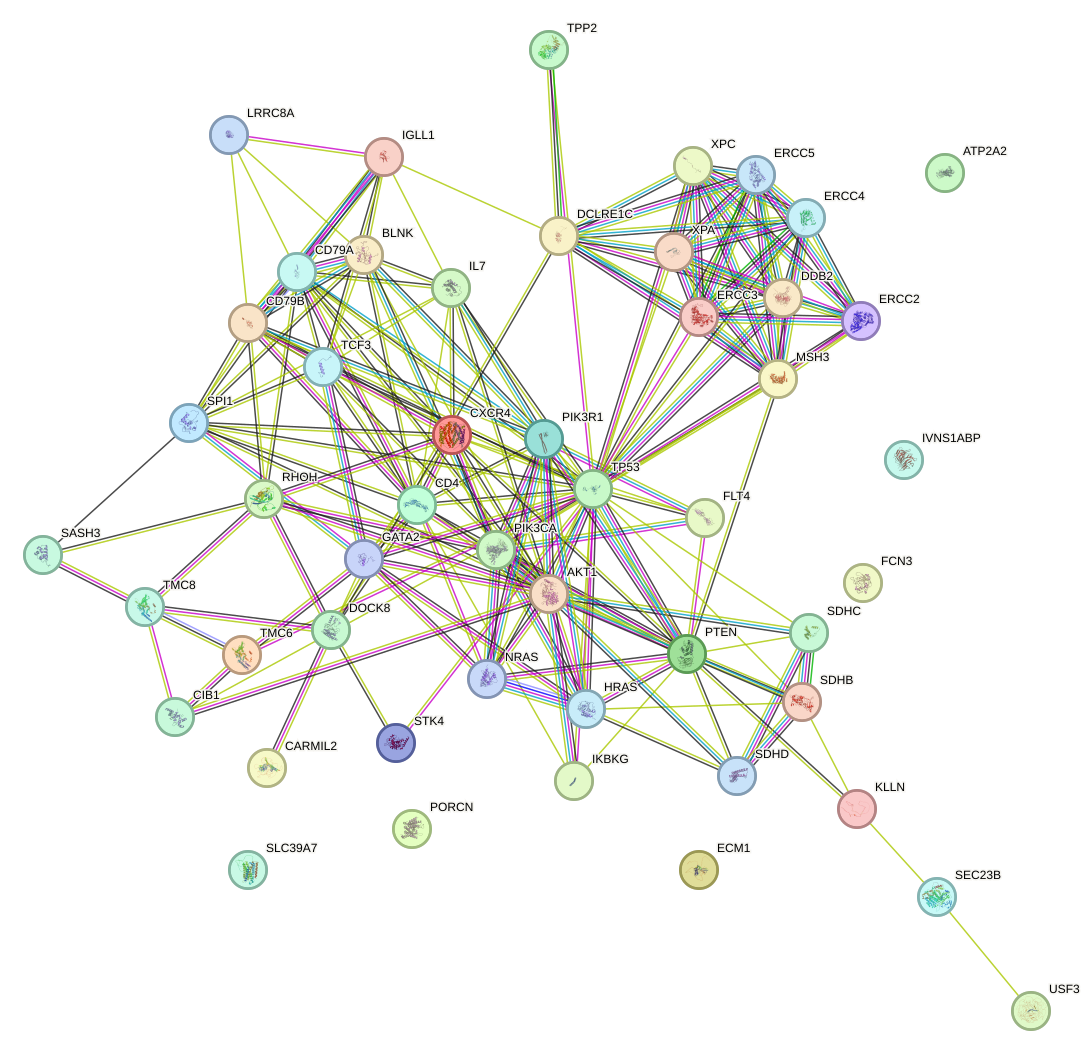
\includegraphics[width=0.8\linewidth]{red_inicial}
	\caption{Red formada por los 51 genes relacionados con el fenotipo \textbf{Papilloma}}
	\label{fig:grado_centralidad}
\end{figure}

\subsection{Análisis de enriquecimiento funcional}

Se realizó un análisis de enriquecimiento funcional destacando las categorías \textbf{Process} y \textbf{KEGG}, obteniendo relaciones entre algunos grupos de genes con problemas del sistema inmune, carcinoma y las adipoquinas.

Los términos y categorías relacionados con enfermedades como \textbf{cervix}, \textbf{ovarian}, \textbf{HPV}, \textbf{herpes}, \textbf{papillomavirus}, \textbf{costellos} y \textbf{cowden} fueron encontrados en el análisis de enriquecimiento funcional, indicando posibles vínculos entre estos términos y los genes asociados al fenotipo estudiado.

Se realizaron búsquedas específicas de genes clave como \textbf{TP53}, \textbf{AKT1}, \textbf{SDHB}, \textbf{SDHD}, \textbf{HRAS} dentro de las categorías significativas. Estos genes podrían tener una importancia particular en relación con el fenotipo de interés, evidenciando su posible relevancia funcional.

\subsection{Descarga y procesamiento de la red de interacción}

Se descargó la red de interacción en formato TSV. El archivo descargado se procesó para dar como resultado un archivo de texto \textbf{$genes_igraph.txt$} formado por dos columnas de nombres de genes, en las que cada fila representa una relación entre dos genes.



\subsection{Propiedades de la red y detección de comunidades}

En nuestra red vimos que todos los nodos estaban conectados entre sí y que se trataba de un grafo no dirigido.

\vspace{3pt}

Obtuvimos una tabla con el \textbf{grado de centralidad} de cada gen. Pudimos observar como el gen de interés TP53 es el que presentaba un mayor grado de centralidad y por tanto más relaciones con otros genes. 
\begin{figure}
	\centering
	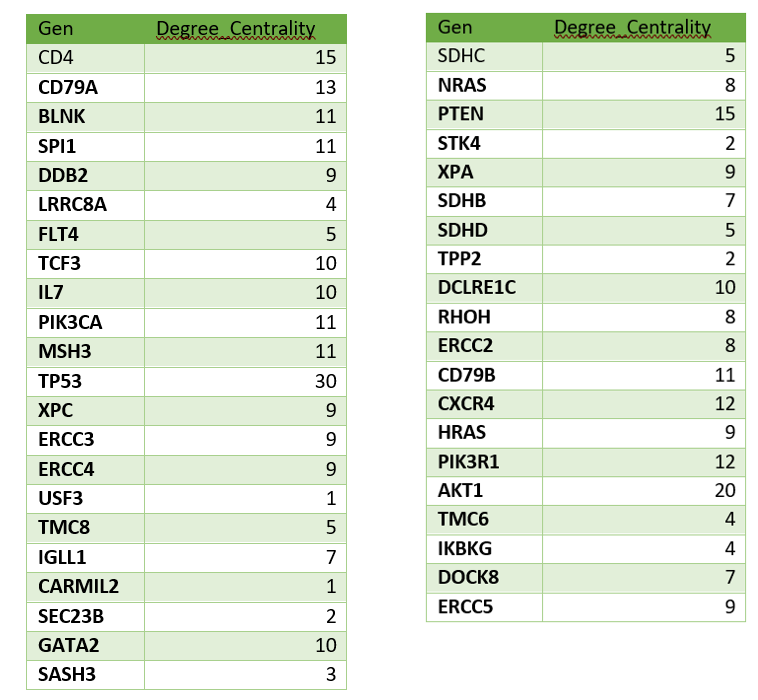
\includegraphics[width=0.8\linewidth]{grado_centralidad}
	\caption{Descripción de la figura.}
	\label{fig:grado_centralidad}
\end{figure}


\vspace{3pt}

En cuanto al \textbf{grado de conectividad} obtuvimos un valor del 19\%, el cual era bastante pequeño y nos indicaba que nuestro grafo no era muy fuerte. Esto puede deberse a que las comunidades entre si no tenían una gran dependencia y teníamos varios genes que no nos interesaban. 

\vspace{3pt}

Empleamos distintos algoritmos para \textbf{detectar comunidades}. En el caso del método de Girvan-Newman había nodos que no pertenecían a ninguna comunidad. Esto podía deberse a la forma en que el algoritmo de betweenness identifica comunidades. Puede detectar comunidades basándose en la centralidad de intermediación de los nodos, y algunos nodos pueden no estar claramente vinculados a una comunidad en función de esta medida.

\vspace{3pt}

Con el algoritmo voraz todos los nodos pertenecían a alguna comunidad. al igual que con el algoritmo de propagación de etiquetas. Sin embargo, en este último obtuvimos tan solo 3 comunidades por lo que la clusterización es mínima.  Con la aplicación del método de Louvain también resultaban menos comunidades que con el algoritmo voraz. Observamos 4 comunidades. 

\begin{figure}
	\centering
	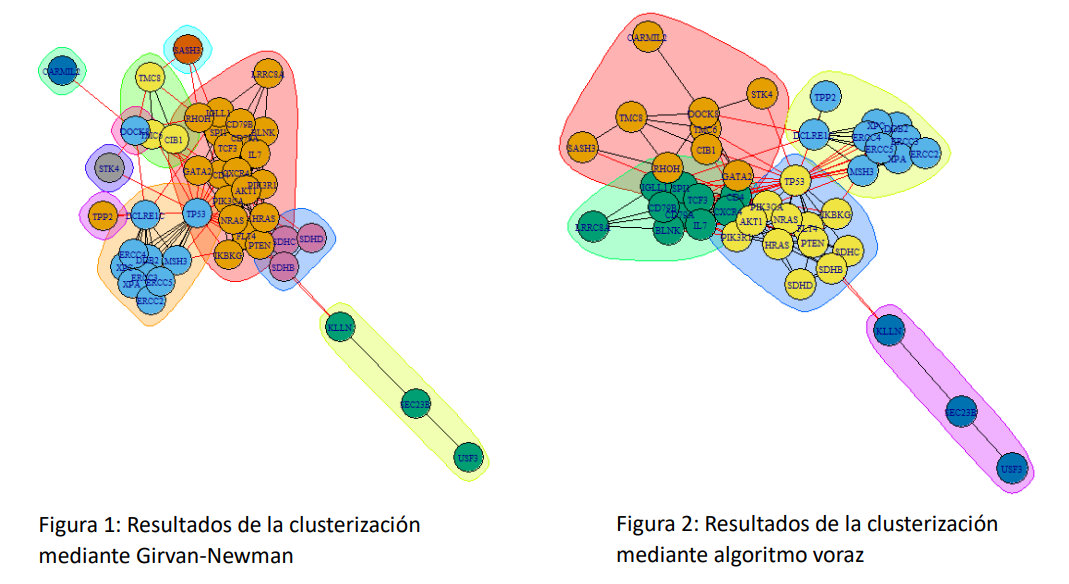
\includegraphics[width=0.8\linewidth]{cluster_GN_voraz}
	\caption{Descripción de la figura.}
	\label{fig:cluster_GN_voraz}
\end{figure} 

\begin{figure}
	\centering
	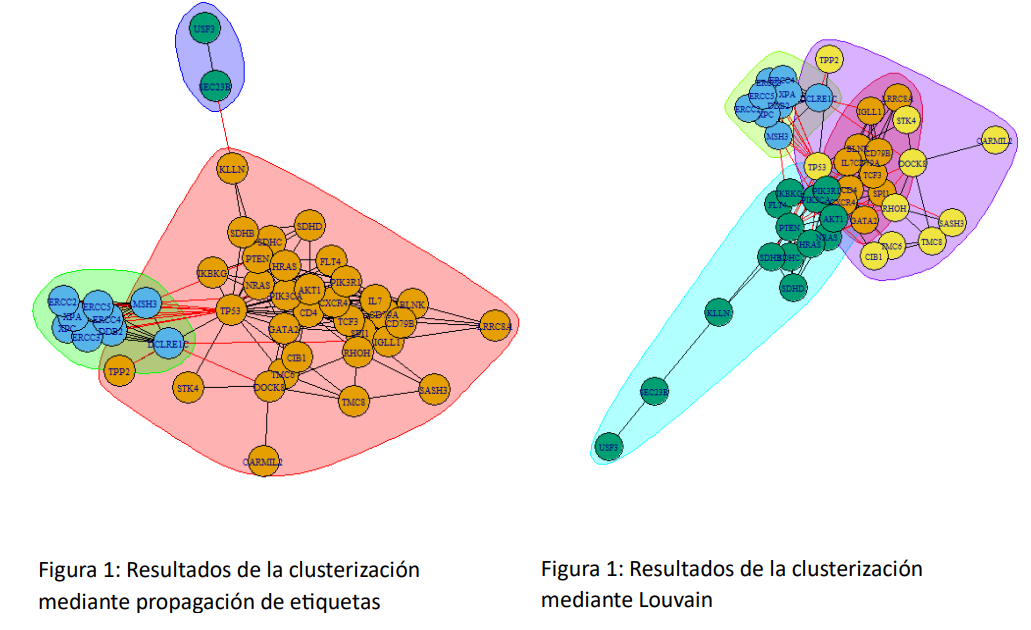
\includegraphics[width=0.8\linewidth]{cluster_etiq_louvain}
	\caption{Descripción de la figura.}
	\label{fig:cluster_etiq_louvain}
\end{figure}

Los algoritmos anteriores tenían la desventaja de que no reflejaban con exactitud la posibilidad de que un gen perteneciera a más de una comunidad. Para estudiar esto hicimos uso de \textbf{Link Communities}, y obtuvimos una gráfica donde cada gen era representado por un diagrama de sectores. Observamos que la mayoría de los genes pertenecen a más de una comunidad. Al centrarnos en nuestros genes de interés detectamos que el gen \textbf{TP53} tenía relación con 4 clusters distintos mientras que los otros genes de interés, SDHB, SDHb,HRAS, AKT1 se encontraban en una comunidad más diferenciada de color rosa. 

\begin{figure}
	\centering
	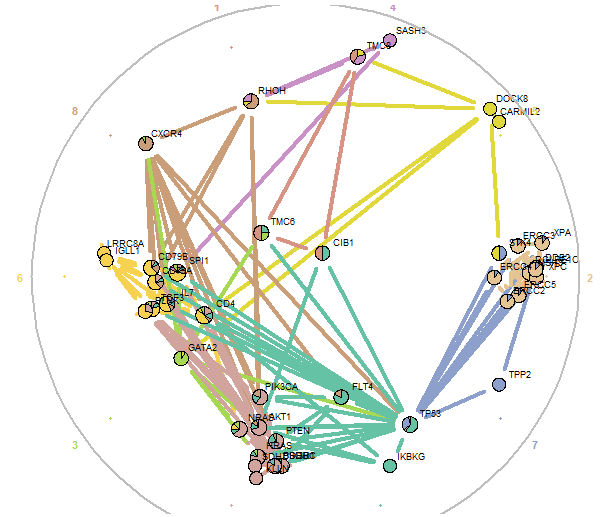
\includegraphics[width=0.8\linewidth]{link}
	\caption{Descripción de la figura.}
	\label{fig:link}
\end{figure}



Para el \textbf{estudio genes de interés} obtuvimos una tabla con dos columnas, el gen en concreto y sus genes vecinos. Observamos que todos los genes estaban relacionados entre sí menos el caso de TP53 y SDHD. 

\begin{figure}
	\centering
	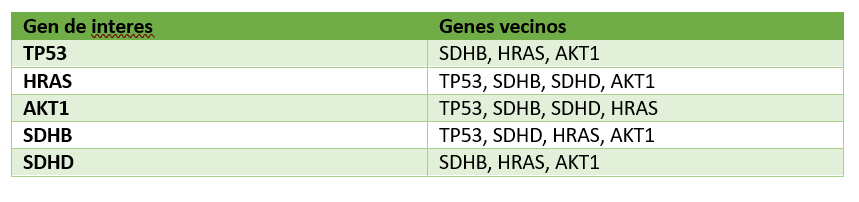
\includegraphics[width=0.8\linewidth]{gen_interes}
	\caption{Descripción de la figura.}
	\label{fig:gen_interes}
\end{figure}

\subsection{Relación de los genes de interés con fenotipos patológicos.}

Tras enriquecer el conjunto de genes de interés hemos obtenido 729 entradas en las cuales hemos encontrado relaciones de genes con fenotipos patológicos como estos:

\begin{table}[h]
	\centering
	\caption{Fenotipos patológicos con palabra clave papiloma}
	\begin{tabular}{|c|c|}
		\hline
		\textbf{Genes} & \textbf{Fenotipos patológicos asociados} \\
		\hline
		FLT4,PIK3CA,TP53,SDHC,NRAS,PTEN,SDHB,SDHD,HRAS,PIK3R1,AKT1,IKBKG & Papiloma \\
		\hline
		TP53,NRAS & Papiloma del plexo coroideo \\
		\hline
	\end{tabular}
\end{table}

\begin{table}[h]
	\centering
	\caption{Fenotipos patológicos con palabra clave papiloma}
	\begin{tabular}{|c|c|}
		\hline
		\textbf{Genes} & \textbf{Fenotipos patológicos genital} \\
		\hline
		PIK3CA,TP53,SDHC,NRAS,PTEN,SDHB,SDHD,AKT1 & Neoplasia genital \\
		\hline
		FLT4,PIK3CA,TP53,SDHC,NRAS,PTEN,SDHB,SDHD,HRAS,AKT1 & Anomalía de los genitales externos masculinos \\
		\hline
		PIK3CA,TP53,SDHC,NRAS,PTEN,SDHB,SDHD,AKT1 & Morfología anormal de los genitales internos femeninos \\
		\hline
	\end{tabular}
\end{table}

\begin{table}[h]
	\centering
	\caption{Fenotipos patológicos con palabra clave renal}
	\begin{tabular}{|c|c|}
		\hline
		\textbf{Genes} & \textbf{Fenotipos patológicos asociados} \\
		\hline
		PIK3CA,TP53,SDHC,NRAS,PTEN,SDHB,SDHD,AKT1 & Neoplasia renal \\
		\hline
		PIK3CA,SDHC,NRAS,PTEN,SDHB,SDHD,AKT1 & Carcinoma de células renales \\
		\hline
		PIK3CA,TP53,SDHC,PTEN,SDHB,SDHD,AKT1 & Anomalía de las glándulas suprarrenales \\
		\hline
		TP53,SDHC,PTEN,SDHB,SDHD & Neoplasia de la glándula suprarrenal \\
		\hline
		SDHC,SDHB,SDHD & Feocromocitoma extraadrenal \\
		\hline
		SDHC,SDHB,SDHD & Feocromocitoma suprarrenal \\
		\hline
	\end{tabular}
\end{table}

\begin{table}[h]
	\centering
	\caption{Fenotipos patológicos con palabra clave carcinoma}
	\begin{tabular}{|c|c|}
		\hline
		\textbf{Genes} & \textbf{Fenotipos patológicos asociados} \\
		\hline
		PIK3CA,SDHC,NRAS,PTEN,SDHB,SDHD,HRAS,AKT1 & Carcinoma folicular de tiroides \\
		\hline
		PIK3CA,TP53,SDHC,NRAS,PTEN,SDHB,SDHD,HRAS,AKT1 & Carcinoma de tiroides \\
		\hline
		PIK3CA,TP53,SDHC,PTEN,SDHB,SDHD,AKT1 & Carcinoma de mama \\
		\hline
		PIK3CA,SDHC,NRAS,PTEN,SDHB,SDHD,AKT1 & Carcinoma de células renales \\
		\hline
		PIK3CA,SDHC,PTEN,SDHB,SDHD,AKT1 & Carcinoma de endometrio \\
		\hline
		PIK3CA,NRAS,PTEN,HRAS,AKT1 & Carcinoma de células transicionales de vejiga \\
		\hline
		PIK3CA,NRAS,AKT1 & Carcinoma colorrectal hereditario no polipósico \\
		\hline
		NRAS,HRAS1 & Carcinoma no medular de tiroides \\
		\hline
		PIK3CA,AKT1 & Adenocarcinoma papilar de ovario \\
		\hline
		PIK3CA,TP53 & Adenocarcinoma de pulmón \\
		\hline
		NRAS,HRAS & Carcinoma papilar de tiroides \\
		\hline
		NRAS,HRAS & Carcinoma basocelular \\
		\hline
		PIK3CA,TP53 & Carcinoma hepatocelular \\
		\hline
		TP53,AKT1 & Carcinoma \\
		\hline
	\end{tabular}
\end{table}

\begin{table}[h]
	\centering
	\caption{Fenotipos patológicos con palabra clave ovario y derivados}
	\begin{tabular}{|c|c|}
		\hline
		\textbf{Genes} & \textbf{Fenotipos patológicos asociados} \\
		\hline
		PIK3CA,TP53,PTEN,AKT1 & Neoplasia ovárica \\
		\hline
		PIK3CA,AKT1 & Adenocarcinoma papilar de ovario \\
		\hline
		PIK3CA,TP53,SDHC,PTEN,SDHB,SDHD,AKT1 & Anomalía del ovario \\
		\hline
		PIK3CA,SDHC,PTEN,SDHB,SDHD,AKT1 & Ovarios poliquísticos agrandados \\
		\hline
	\end{tabular}
\end{table}

\begin{table}[h]
	\centering
	\caption{Fenotipos patológicos con palabra clave útero y derivados}
	\begin{tabular}{|c|c|}
		\hline
		\textbf{Genes} & \textbf{Fenotipos patológicos asociados} \\
		\hline
		PIK3CA,SDHC,NRAS,PTEN,SDHB,SDHD,AKT1 & Neoplasia uterina \\
		\hline
		PIK3CA,NRAS,AKT1 & Leiomiosarcoma uterino \\
		\hline
		FLT4,SDHB,SDHD,PIK3R1 & Retraso del crecimiento intrauterino \\
		\hline
	\end{tabular}
\end{table}
\clearpage

	\section{Discusión}

El estudio presenta un análisis exhaustivo de la red de genes asociados al fenotipo Papiloma, abordando aspectos clave que van desde la identificación de genes hasta la exploración de relaciones con fenotipos patológicos. A continuación, se discuten las implicaciones y hallazgos más relevantes del estudio.

\vspace{3pt}

En el estudio de red de interacción entre genes (sección 3.1), se destaca la identificación de 51 genes vinculados al fenotipo Papiloma. La representación visual de la red de interacción ofrece una visión intuitiva de cómo estos genes están conectados entre sí.

\vspace{3pt}

El análisis de enriquecimiento funcional (sección 3.2) profundiza en la funcionalidad de los genes identificados y la participación común de estos en vías metabólicas del sistema inmune, afectadas por carcinomas y relacionadas con el síndrome de Costellos y Cowden.  En particular, los vínculos encontrados del gen HRAS con la enfermedad de costellos concuerda con los hallazgos de otros autores, que postulan como mutaciones de dicho gen, que regula vías de transducción, tienen una gran relación con la enfermedad \cite{Siegel2012}.  Nuestros hallazgos también confirman lo evidenciado por otros científicos, en cuanto a como el cancer de endometrio se ha reconocido como uno de los componentes del síndrome de Cowden debido a alteraciones en las líneas germinales de PTEN y SDHB-D \cite{Mahdi2015}.
	\section{Conclusiones}
El estudio proporciona una interesante red de genes asociados al fenotipo Papiloma, desde la identificación de la interacción de estos hasta su implicación en distintos fenotipos patológicos. Este estudio ofrece una información valiosa para la comunidad científica y médica. Desde una perspectiva médica, la identificación de genes clave y sus interacciones proporciona importante información para el diagnóstico, tratamiento y desarrollo de terapias dirigidas relacionadas con el fenotipo patológico estudiado. Desde un punto de vista científico, este trabajo contribuye al entendimiento más profundo de la relación entre la genética y el desarrollo de fenotipos específicos, en nuestro caso, el Papiloma. Además la investigación aporta información sobre la utilización y enfoque de algoritmos sobre el análisis de redes.

	
	
	%%%%%%%%%%%%%%%%%%%%%%%%%%%%%%%%%%%%%%%%%%%%%%
	%% OTRA INFORMACIÓN                         %%
	%%%%%%%%%%%%%%%%%%%%%%%%%%%%%%%%%%%%%%%%%%%%%%
	
	\begin{backmatter}
	
		\section*{Abreviaciones}%% if any
			Indicar lista de abreviaciones mostrando cada acrónimo a que corresponde
		
		\section*{Disponibilidad de datos y materiales}%% if any
			Debéis indicar aquí un enlace a vuestro repositorio de github.
		
		\section*{Contribución de los autores}
			Usando las iniciales que habéis definido al comienzo del documento, debeis indicar la contribución al proyecto en el estilo:
			J.E : Encargado del análisis de coexpresión con R, escritura de resultados; J.R.S : modelado de red con python y automatizado del código, escritura de métodos; ...
			OJO: que sea realista con los registros que hay en vuestros repositorios de github. 
		
		
		%%%%%%%%%%%%%%%%%%%%%%%%%%%%%%%%%%%%%%%%%%%%%%%%%%%%%%%%%%%%%%%%%%%%%%%%%%%%%%%%%%%%%%%%
		%% BIBLIOGRAFIA: no teneis que tocar nada, solo sustituir el archivo bibliography.bib %%
		%% por el que hayais generado vosotros                                                %%
		%%%%%%%%%%%%%%%%%%%%%%%%%%%%%%%%%%%%%%%%%%%%%%%%%%%%%%%%%%%%%%%%%%%%%%%%%%%%%%%%%%%%%%%%
		
		\bibliographystyle{bmc-mathphys} % Style BST file (bmc-mathphys, vancouver, spbasic).
		\bibliography{bibliography}      % Bibliography file (usually '*.bib' )
	
	\end{backmatter}
\end{document}
